%Use 16:9
\documentclass[dvipsnames]{beamer}
\usepackage{graphicx} % Required for inserting images
\usepackage{xcolor}
\definecolor{codebg}{HTML}{0D1117} % GitHub Dark background
\usepackage[newfloat]{minted}
\usepackage{fontspec}
\setmonofont{Fira Code}
% Colors
\usepackage{xcolor}

% Use the same style everywhere
\usemintedstyle{monokai}

% Global minted defaults (including background)
\setminted{
  breaklines,
  breakanywhere,
  linenos,
  numbersep=6pt,
  fontsize=\footnotesize,
  xleftmargin=1em,
  tabsize=2,
  bgcolor=codebg,             % <<< make minted's background dark
}

% C++-specific tweaks
\setminted[c++]{
  mathescape,
  escapeinside=||,
}


% Make line numbers readable on dark bg (optional but nice)
\makeatletter
\renewcommand\theFancyVerbLine{%
  \textcolor{white!60}{\arabic{FancyVerbLine}}%
}
\makeatother

% tcolorbox wrapper: use the same background + a subtle frame
\usepackage[most]{tcolorbox}
\tcbuselibrary{minted,skins,breakable}
\newtcblisting{cppcode}[1][]{
  listing engine=minted,
  minted language=c++,
  minted style=monokai,  % keep in sync
  minted options={
    linenos,autogobble,breaklines,fontsize=\footnotesize,
    mathescape,escapeinside=||,
 %   bgcolor=codebg,          % <<< align inner bg with the box
  },
%  colback=codebg,            % <<< box background
  colframe=white!10,         % subtle border against black
  enhanced, breakable,
  boxrule=0.4pt, arc=2.5pt,
  left=1em, right=1em, top=0.6em, bottom=0.6em,
  borderline west={2.2pt}{0pt}{blue!65!black}, % accent stripe
  #1
}
\usepackage{mathtools}
\usepackage[thinc]{esdiff}
\usepackage{tikz}
\usetikzlibrary{shapes,arrows,positioning}
\usetikzlibrary{calc}
\usepackage{listings}
\usepackage{tikz}
\usetikzlibrary{shapes, arrows.meta, positioning}
\usepackage{animate}
% --- Minimal 64B cache line utilities ---------------------------------------
% Requires: \usepackage{tikz} \usetikzlibrary{arrows.meta}

% Environment draws an 8-block bar; you add colors/marks inside it.
\newenvironment{CacheLine}[1][]{
  \begin{tikzpicture}[x=1.2cm,y=0.8cm,font=\footnotesize,>=Stealth,#1]
    % Geometry knobs (in "y units"); tweak with \CacheSetBelow if needed.
    \def\CacheH{1.0}   % bar height
    \def\CacheBelow{1.0} % how far below the bar the bottom labels sit

    % (We fill blocks and draw marks here; lines/labels go at the end)
}{
    % Vertical dividers and labels (drawn last so they sit on top of fills)
    \foreach \i in {1,...,7} { \draw[black!40] (\i,0) -- (\i,\CacheH); }
    \draw[line width=0.6pt, rounded corners=2pt] (0,0) rectangle (8,\CacheH);
    \foreach \i in {0,...,7} {
      \node[below=3pt, text=black!75] at (\i+0.5,0) {8B \i};
    }
  \end{tikzpicture}
}

% Color a single 8B block i with a given color (keeps lines visible via opacity)
% Usage: \CacheColor{<i 0..7>}{<color>}
\newcommand{\CacheColor}[2]{%
  \fill[#2, fill opacity=0.35, draw=none] (#1,0) rectangle ++(1,\CacheH);%
}

% Color a contiguous range of blocks [i,j) (e.g., 2..5 colors blocks 2,3,4)
% Usage: \CacheColorRange{<i>}{<j>}{<color>}
\newcommand{\CacheColorRange}[3]{%
  \fill[#3, fill opacity=0.35, draw=none] (#1,0) rectangle (#2,\CacheH);%
}

% Mark the START (left edge) of block i with an arrow and label ABOVE.
% Usage: \CacheMarkAbove[<color>]{<i 0..7>}{<label>}
\newcommand{\CacheMarkAbove}[3][green!60!black]{%
  \draw[-{Stealth[length=3mm]}, very thick, draw=#1] (#2,\CacheH+0.36) -- (#2,\CacheH+0.04);
  \node[above, text=#1] at (#2,\CacheH+0.36) {#3};
}

% Mark the START (left edge) of block i with an arrow and label BELOW.
% (Moved further down so it clears the "8B k" tick labels.)
% Usage: \CacheMarkBelow[<color>]{<i 0..7>}{<label>}
\newcommand{\CacheMarkBelow}[3][green!60!black]{%
  \draw[-{Stealth[length=3mm]}, very thick, draw=#1] (#2,-\CacheBelow+0.28) -- (#2,0.02);
  \node[below, text=#1] at (#2,-\CacheBelow+0.28) {#3};
}

% Optional: adjust how far below the bar the bottom labels/arrows go (in "y units")
% e.g., \CacheSetBelow{1.2} pushes them farther down.
\newcommand{\CacheSetBelow}[1]{\def\CacheBelow{#1}}
% ---------------------------------------------------------------------------

\title{Reverse Mode Automatic Differentiation: Unraveling Expression Graphs \& Library Magic}
\author{Steve Bronder}
\date{October 2023}

\def\mathcolor#1#{\@mathcolor{#1}}
\def\@mathcolor#1#2#3{%
  \protect\leavevmode
  \begingroup
    \color#1{#2}#3%
  \endgroup
}

\newcommand{\fracp}[2]{\frac{\partial #1}{\partial #2}}
\newcommand{\pp}[2]{\frac{\partial#1}{\partial#2}}
\newcommand{\adj}[1]{\bar{#1}}
\newcommand{\pluseq}{\mathrel{+}=}

\makeatother

\begin{document}
\expandafter\def\expandafter\insertshorttitle\expandafter{%
  \insertshorttitle\hfill%
  \insertframenumber\,/\,\inserttotalframenumber}
\maketitle
% Slide


{ % all template changes are local to this group.
    \setbeamertemplate{navigation symbols}{}
    \begin{frame}<article:0>[plain]
        \begin{tikzpicture}[remember picture,overlay]
            \node[at=(current page.center)] {
                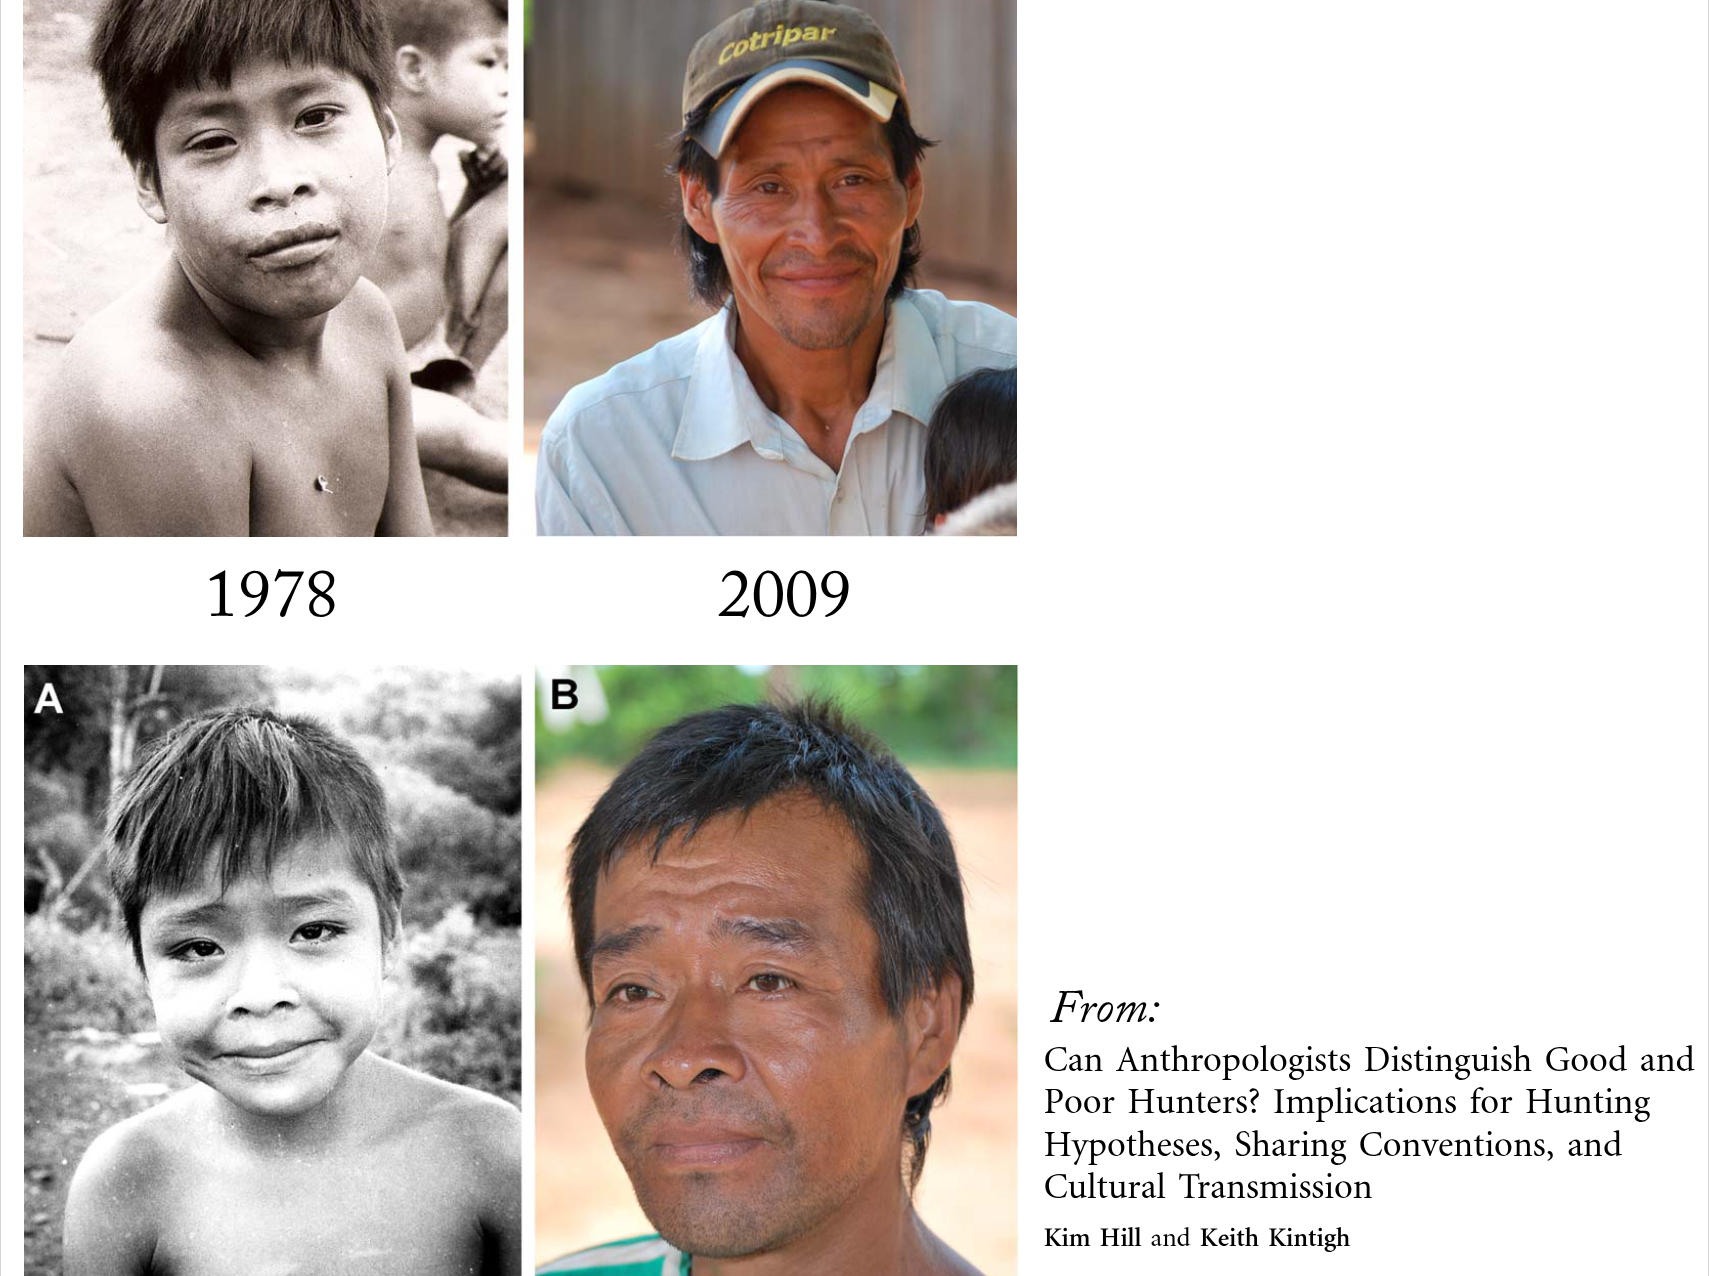
\includegraphics[keepaspectratio,
                                 width=\paperwidth,
                                 height=\paperheight]{img/mcel1.png}
            };
        \end{tikzpicture}
     \end{frame}
}

{ % all template changes are local to this group.
    \setbeamertemplate{navigation symbols}{}
    \begin{frame}<article:0>[plain]
        \begin{tikzpicture}[remember picture,overlay]
            \node[at=(current page.center)] {
                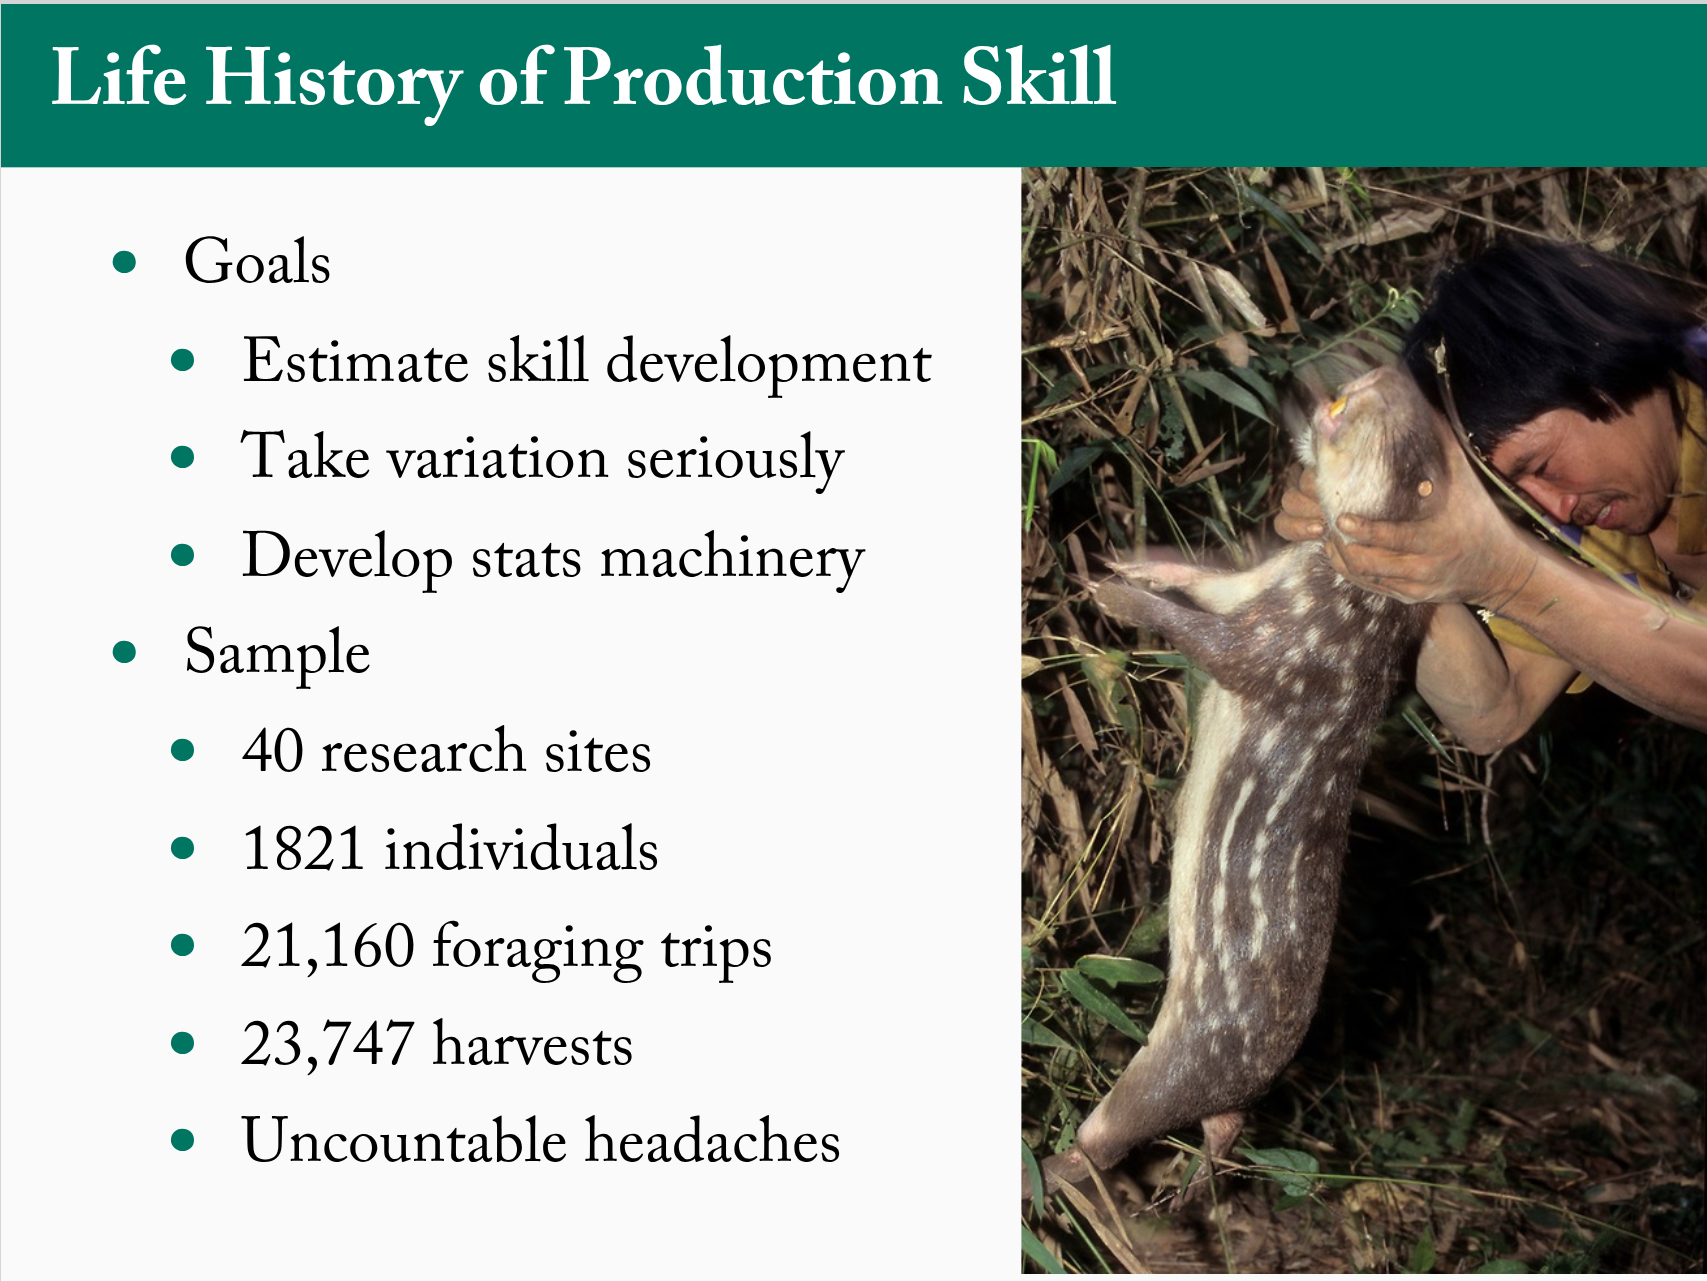
\includegraphics[keepaspectratio,
                                 width=\paperwidth,
                                 height=\paperheight]{img/mcel2.png}
            };
        \end{tikzpicture}
     \end{frame}
}

{ % all template changes are local to this group.
    \setbeamertemplate{navigation symbols}{}
    \begin{frame}<article:0>[plain]
        \begin{tikzpicture}[remember picture,overlay]
            \node[at=(current page.center)] {
                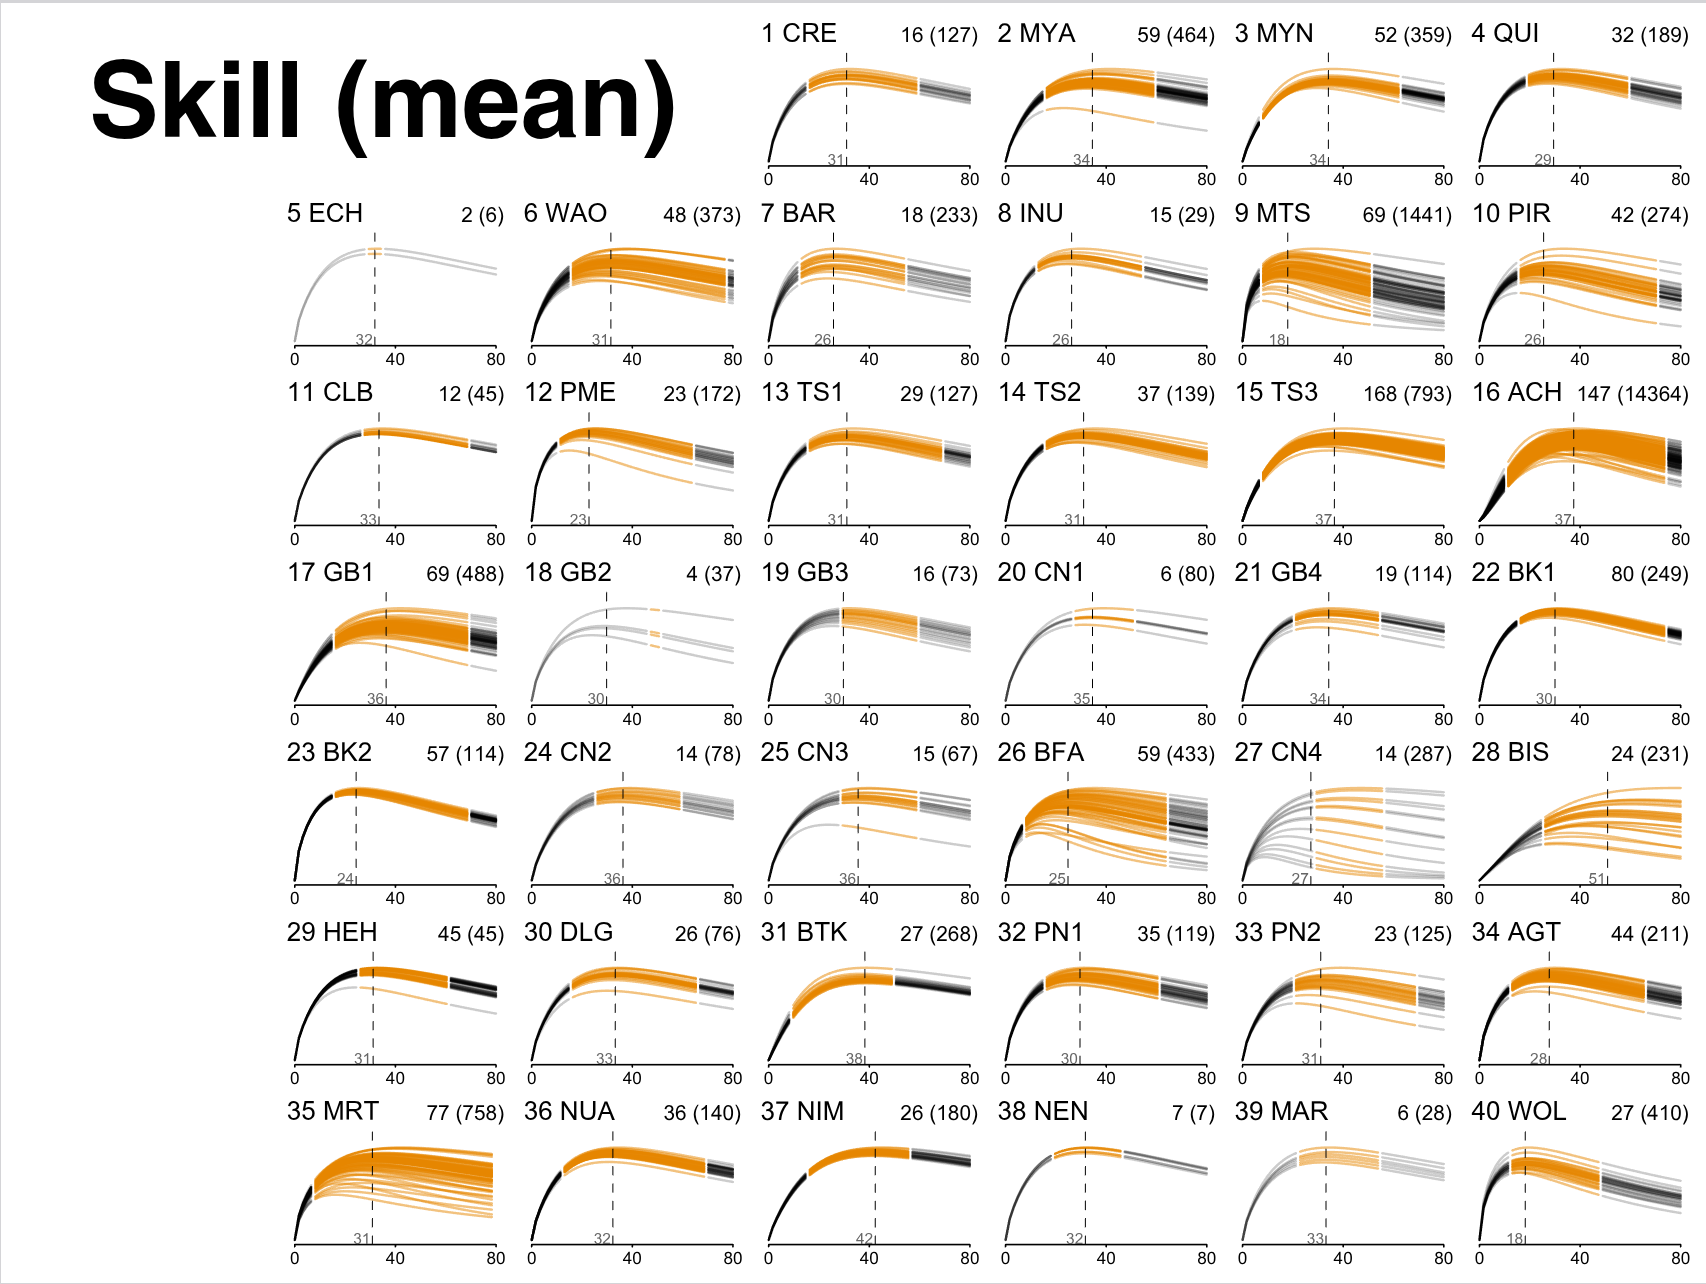
\includegraphics[keepaspectratio,
                                 width=\paperwidth,
                                 height=\paperheight]{img/mcel3.png}
            };
        \end{tikzpicture}
     \end{frame}
}

\begin{frame}{Estimating COVID Infection Rates For Policy}
\begin{figure}
\centerline{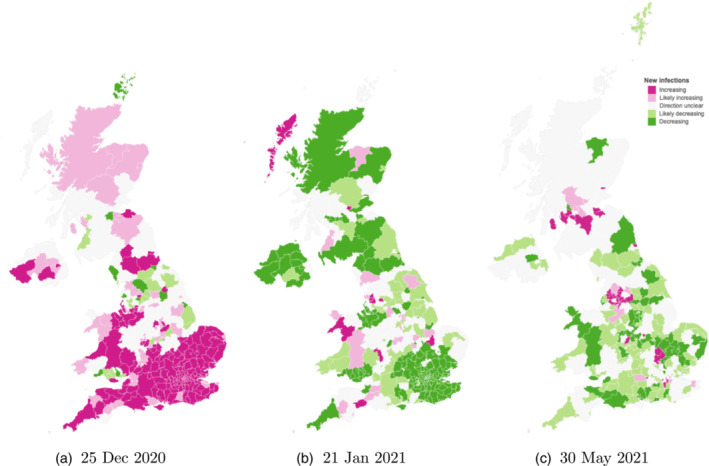
\includegraphics[scale=.5]{img/covid_uk.jpg}}
\caption{Probability of epidemic growth by local area}
\label{fig-covid}
\end{figure}
\end{frame}

\note{These models can only exist because autodiff exists}
\begin{frame}{Automatic Differentiation Probably Effects Your Day to Day}
\begin{figure}
\centerline{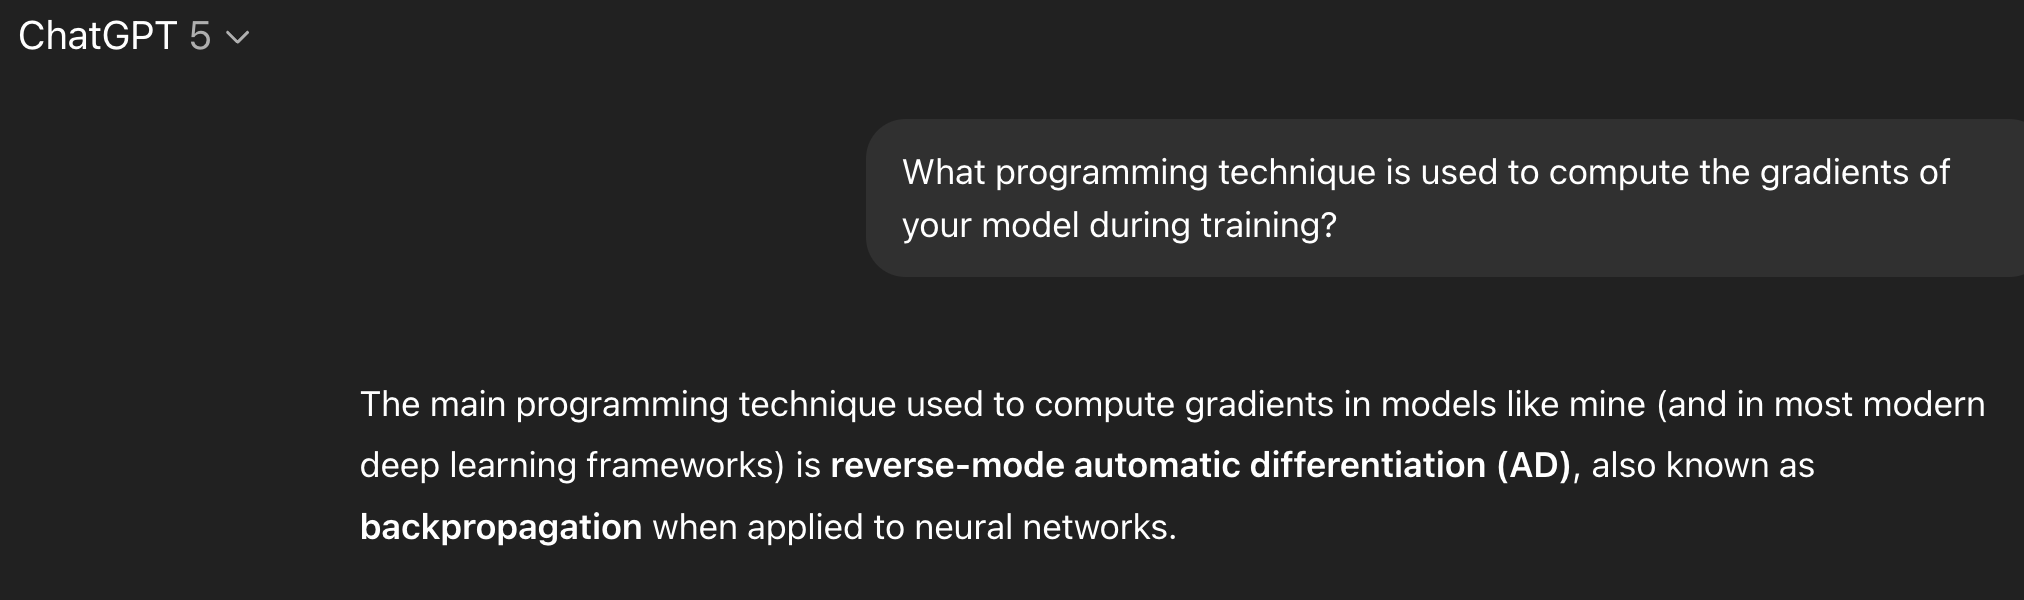
\includegraphics[scale=.16]{img/chatgpt.png}}
\label{fig-chatgpt}
\end{figure}
\end{frame}

\note{Autodiff is the mitochondria of machine learning. AD allows for efficient estimation of many statistical models.}

\begin{frame}{What's Automatic Differentiation?}
 Computational technique for evaluating derivatives of functions expressed as computer programs by systematically applying the chain rule.
\begin{figure}
\centerline{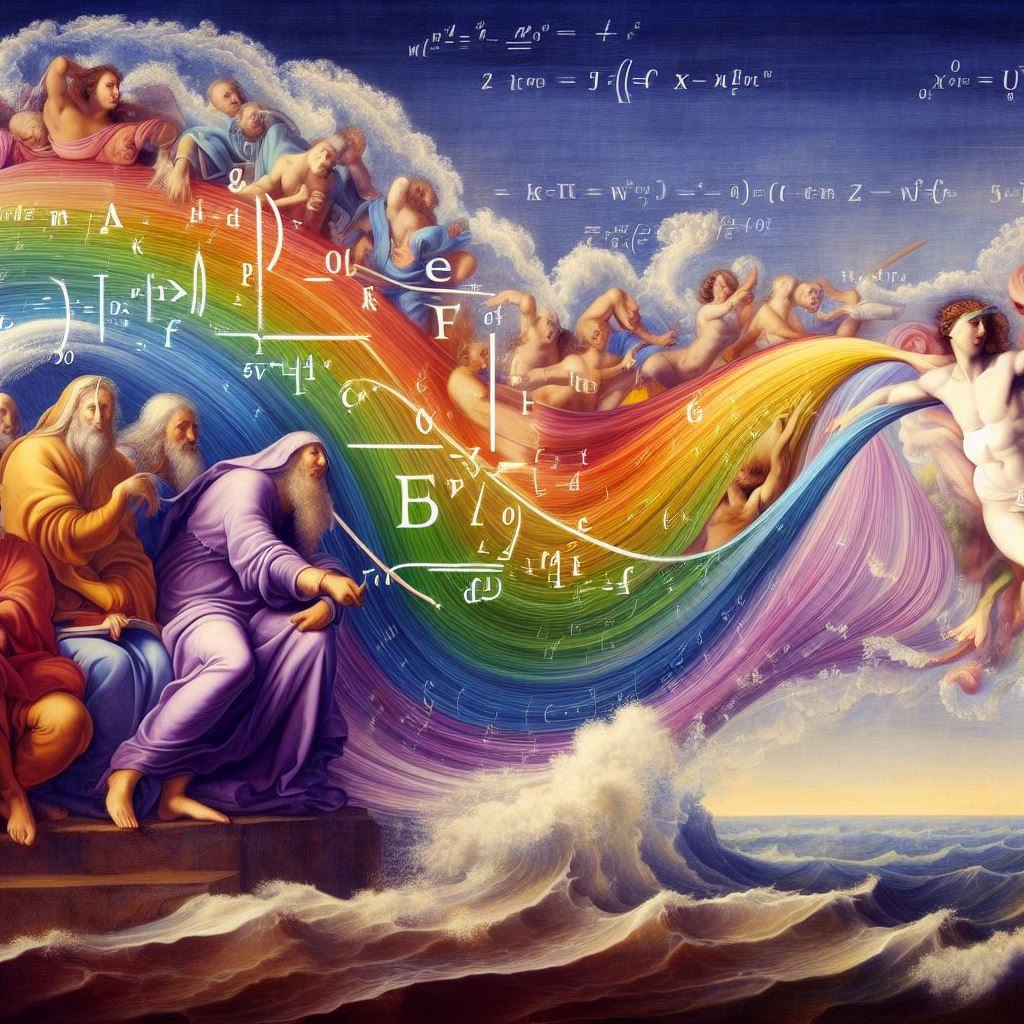
\includegraphics[scale=.15]{img/image.png}}
\caption{Asking ChatGPT to make a physical representation of automatic differentiation.}
\label{fig-delulu}
\end{figure}
\vspace{-7mm}
\end{frame}

\begin{frame}{Why use Automatic Differentiation?}
Ex: Newton's method for finding root of function (where output is 0)

\begin{equation*}
    x_{n+1} = x_n - \frac{f\left(x_n\right)}{f'\left(x_{n}\right)}
\end{equation*}

\end{frame}

\note{How do we estimate solutions for equations? A simple method is the newton method.

Why are gradients useful? We use gradients to solve

For models we want to estimate parameter values. Change the slide here so that we show how to solve for parameters using newtons method}

\begin{frame}{Why use Automatic Differentiation?}
\begin{align}
    f(x) &= x^3 + x^2 + x\\
    f'(x) &= 3x^2 + 2x + 1
\end{align}
\centering
\animategraphics[loop,controls,scale=0.35]{2}{gif/newton-}{0}{17}
\end{frame}

\begin{frame}{Why use Automatic Differentiation?}
Think about HMC, BFGS, SGD, etc.
\begin{itemize}
    \item HMC: $\frac{dp}{dt}=-\nabla_\theta\log p(\theta|y)$
    \item BFGS: $s_k=-H_k \nabla_\theta f(\theta_k)$
    \item SGD: $\theta_{t+1}=\theta_t−\eta\nabla_\theta L(\theta_t;x_t)$
\end{itemize}
\begin{itemize}
    \item Choices
    \begin{itemize}
        \item Write by hand
        \item finite difference,
        \item symbolic differentiation
        \item spectral differentiation
        \item automatic differentiation
    \end{itemize}
\end{itemize}

\end{frame}

\begin{frame}{Why use Automatic Differentiation?}

\tiny
\begin{align*}
&\underbrace{p\!\left(
\boldsymbol{\theta} \,\big|\, \mathbf y
\right)}_{\textbf{posterior}}
\;\propto\;
\prod_{i=1}^{N}
\Bigg\{
\sum_{\mathbf z_i \in \{1,2,3\}^{T_i}}
\!\Bigg[
\underbrace{\pi_{z_{i,1}}\prod_{t=2}^{T_i}\Pi_{z_{i,t-1},\,z_{i,t}}}_{\text{3-state HMM prior}}
\;
\prod_{t=1}^{T_i}
\underbrace{\mathcal N\!\Big(
y_{i,t}\,\Big|\,\eta_{i,t},\,\sigma_{z_{i,t}}^{2}
\Big)}_{\text{state-dependent emission}}
\Bigg]
\Bigg\}
\\[-2pt]
&\text{where}\quad
\eta_{i,t}
=\underbrace{\mathbf x_{i,t}^{\!\top}\boldsymbol\beta}_{\text{fixed}}
+\underbrace{\mathbf z^{(G)}_{i,t}{}^{\!\top}\mathbf b_{g[i]}
+\mathbf z^{(C)}_{i,t}{}^{\!\top}\mathbf c_{c[i]}
+u_{g[i]}}_{\text{crossed random effects}}
+\underbrace{f(t_{i,t})}_{\text{GP}}
+\underbrace{\mu_{z_{i,t}}
+\mathbf r_{z_{i,t}}^{\!\top}\mathbf w_i}_{\text{state-specific offset + slope}}
,\qquad z_{i,t}\in\{1,2,3\}.
\\[4pt]
&
p(\mathbf f\mid\boldsymbol\psi)
=
(2\pi)^{-T/2}\,|\mathbf K|^{-1/2}\;
\exp\!\Big(-\tfrac12\,\mathbf f^{\!\top}\mathbf K^{-1}\mathbf f\Big),
\\[-2pt]
&
\mathbf K
=\sigma_f^{2}\Big(\mathbf K_{\text{LP}}(\ell,p,\lambda)\;+\;\rho\,\mathbf K_{\text{SE}}(\tilde\ell)\Big)
+\sigma_n^{2}\mathbf I,\quad
\big[\mathbf K_{\text{LP}}\big]_{t t'}
=\exp\!\left(
-\frac{(t-t')^{2}}{2\ell^{2}}
-\frac{2\sin^{2}\!\big(\pi|t-t'|/p\big)}{\lambda^{2}}
\right),
\\[-2pt]
&
\big[\mathbf K_{\text{SE}}\big]_{t t'}
=
\exp\!\left(-\frac{(t-t')^{2}}{2\tilde\ell^{2}}\right),
\qquad
\mathbf K=\mathbf L_K\mathbf L_K^{\!\top}
\;\Rightarrow\;
\log|\mathbf K|=2\sum_{j=1}^{T}\log \big((\mathbf L_K)_{jj}\big).
\\[6pt]
&\textbf{Hierarchical mixed effects (non-centered, LKJ prior):}
\\[-2pt]
&\qquad
\mathbf b_{g}=\big(\mathbf I_{p_G}\otimes\operatorname{diag}(\boldsymbol\tau_b)\,\mathbf L_R\big)\,\tilde{\mathbf b}_{g},
\;\;
\tilde{\mathbf b}_{g}\sim\mathcal N(\mathbf 0,\mathbf I),
\;\;
\mathbf c_{c}=\operatorname{diag}(\boldsymbol\tau_c)\,\tilde{\mathbf c}_{c},
\;\;
\tilde{\mathbf c}_{c}\sim\mathcal N(\mathbf 0,\mathbf I),
\\[-2pt]
&\qquad
\operatorname{LKJ}_{p_G}(\eta)\ \text{prior on}\ \mathbf R,\quad
\mathbf L_R\mathbf L_R^{\!\top}=\mathbf R,
\quad
\boldsymbol\tau_b\sim\prod_{j=1}^{p_G}\text{Half-}t_{\nu_b}(0,s_b),
\quad
\boldsymbol\tau_c\sim\prod_{j=1}^{p_C}\text{Half-}t_{\nu_c}(0,s_c),
\\[-2pt]
&\qquad
u_g\sim\mathcal N(0,\sigma_u^2).
\end{align*}


\end{frame}
\begin{frame}{Why use Automatic Differentiation?}
\begin{itemize}
\item Faster than finite difference, more flexible than symbolic differentiation
\item Allows for unknown length while and for loops
\item Accurate to floating point precision
\item Reverse Mode AD can compute partials derivatives of inputs at the same time
\end{itemize}
\end{frame}

\begin{frame}{How Fast is AutoDiff?}
\begin{figure}
\centerline{
\includegraphics[scale=.5]{img/mocking-spongebob.jpg}}
\caption{AuToDiFf rUnS iN $\Theta(C(f))$ TiMe}
\label{fig-spongebob}
\end{figure}
\end{frame}

\begin{frame}{Impl Matters!}
\begin{figure}
\centerline{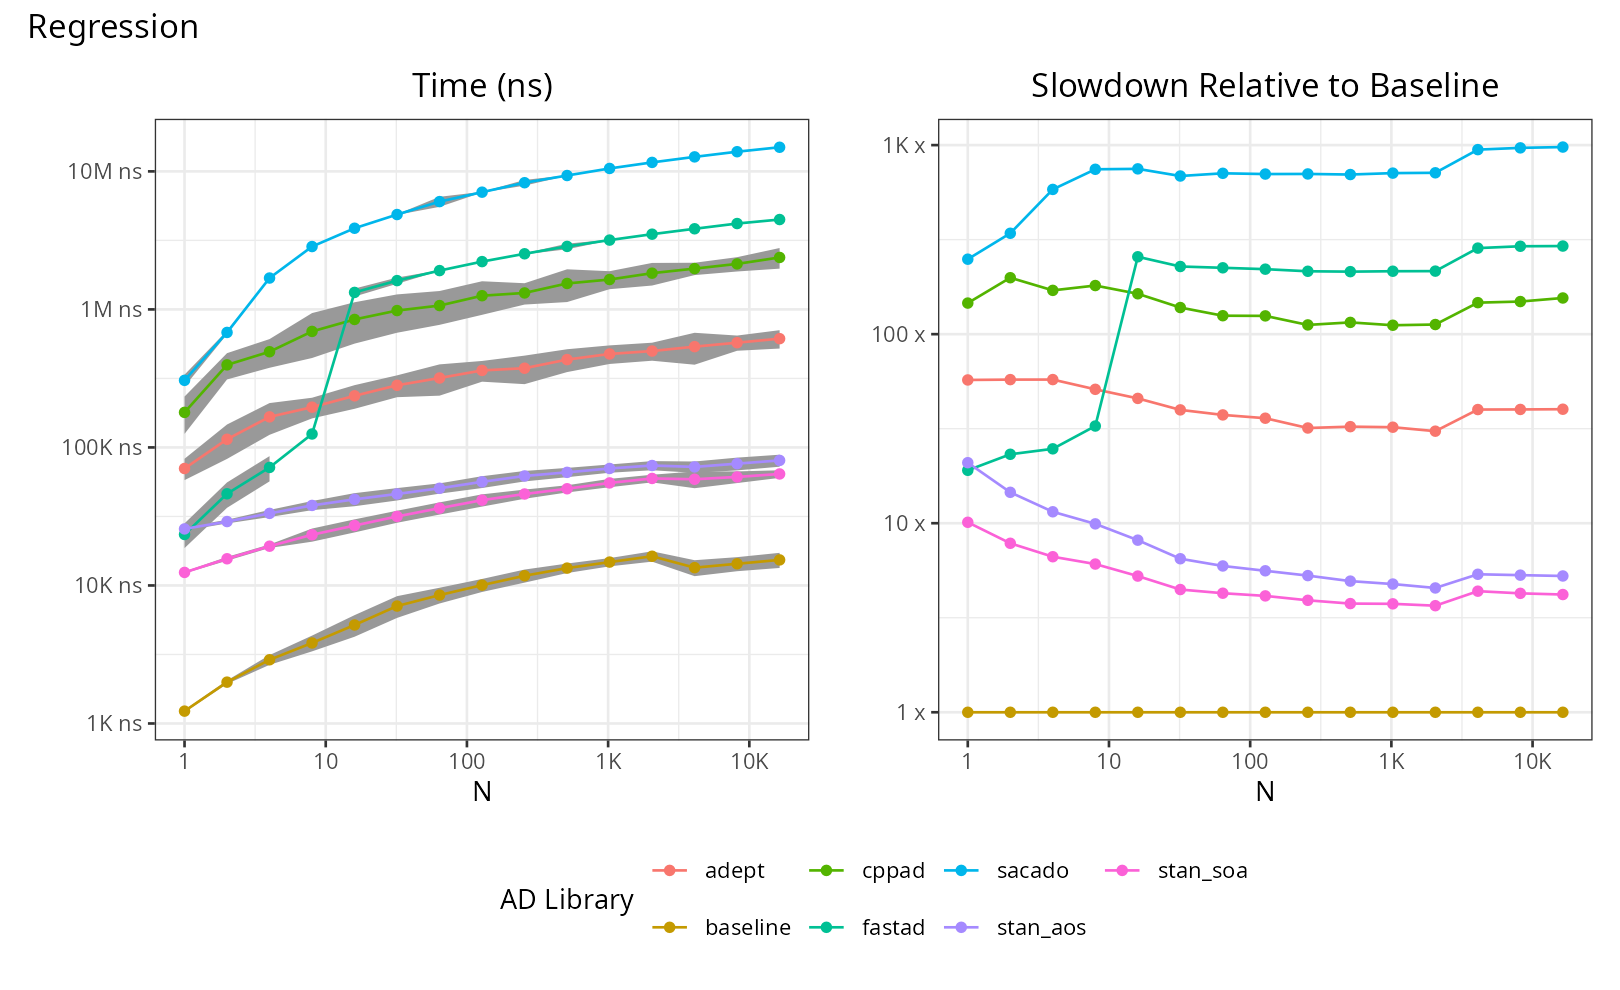
\includegraphics[scale=.5]{img/combined_regression_plot.png}}
\caption{Benchmark for $f'$ given $f = y\sim N(X\theta,\sigma)$}
\label{fig-red-bench}
\end{figure}
\end{frame}

\begin{frame}{Goal of this talk}
\begin{itemize}
    \item Understand performance of high throughput memory intensive programs
    \item Show how modern C++ through time has led to cleaner and more efficient AD
\end{itemize}
\end{frame}

\note{Let $v_k$ be the sequence of intermediate expressions for the input $x$ and output $z$ and let $v_K = z$ and $v_0 = x_0; v_1 = x_1$. Let $\overline{v}_k$ be the partial gradient of the kth intermediate step. Then we can apply the chain rule to each intermediate step to get the partial gradient.
}

\begin{frame}{What's Automatic Differentiation?}

\begin{itemize}
    \item Given a function $f$ with inputs $x\in\mathbb{R}^n$ and outputs $z\in \mathbb{R}^m$ we want to calculate the Jacobian $J$ with size $(m, n)$
    \item To get the full Jacobian, use the chain rule to differentiate from each output to each input.
\end{itemize}


\begin{equation*}
    J_{i, 1:j} = \left\{\fracp{z_i}{x_1}, \cdots, \fracp{z_i}{x_j}\right\}
\end{equation*}

Automatic Differentiation can do higher order partials, but here we just focus on the Jacobian

\end{frame}

\begin{frame}{Cool Math, but how do we do this in a computer??}

 For Reverse Mode AD, we perform two functions.

\begin{itemize}
 \item Forward Pass:
 \begin{equation*}
     z = f(x_0, x_1)
 \end{equation*}
 \item Reverse Pass: Given $z$'s adjoint (gradient) $\overline{z}$
 \begin{equation*}
 chain(z, x_0, x_{1}) = \left\{\diffp{z}{{x_0}}\overline{z},\diffp{z}{{x_1}}\overline{z}\right\}
 \end{equation*}
 \\Calculate the adjoint-jacobian update for $x_0$ and $x_1$.
 \item The calculations needed are represented as an expression Graph
\end{itemize}
\end{frame}

\begin{frame}{What's an Expression Graph?}
 \begin{itemize}
     \item Dependency graph of intermediate computations
     \item Think of both data and operations as objects
     \item Do a forward pass to calculate the values of the intermediates, then a reverse pass to calculate the adjoint-jacobian updates.
 \end{itemize}
 \end{frame}

% Slide 1
\begin{frame}{Forward Pass}
\vspace{-1mm}
$$z = \log(x*y)$$

\begin{tikzpicture}
  [
    Round/.style={circle, draw=black!, fill=green!0, thick, minimum size=2mm},
    Red/.style={circle, draw=black!, fill=red!255, thick, minimum size=2mm},
    Yellow/.style={circle, draw=black!, fill=yellow!255, thick, minimum size=10mm},
    Gray/.style={circle, draw=black!, fill=gray!35, thick, minimum size=2mm}
  ]
  % Nodes
  \node[Gray] (v0) at(-8, 0) {$y$};

  \node[Gray] (v1) at(0, 0) {$x$};

  \node[Round] (v2) at(-4, -2) {$*$};

  \node[Round] (v3) at(-6, -4) {$\log$};



  % Lines
  \path [<-, draw, thick] (v2) -- (v0);
  \path [<-, draw, thick] (v2) -- (v1);
  \path [<-, draw, thick] (v3) -- (v2);

\end{tikzpicture}
\end{frame}

\begin{frame}{Forward Pass}
\vspace{-1mm}
$$z = \log(\mathcolor{red}{x} * \mathcolor{red}{y})$$

\begin{tikzpicture}
  [
    Round/.style={circle, draw=black!, fill=green!0, thick, minimum size=2mm},
    Red/.style={circle, draw=black!, fill=red!255, thick, minimum size=2mm},
    Yellow/.style={circle, draw=black!, fill=yellow!255, thick, minimum size=10mm},
    Gray/.style={circle, draw=black!, fill=gray!35, thick, minimum size=2mm}
  ]
  % Nodes
  \node[Gray, label=left:{\textcolor{blue}{$v_0$}}] (v0) at(-8, 0) {$\mathcolor{red}{y}$};

  \node[Gray, label=left:{\textcolor{blue}{$v_1$}}] (v1) at(0, 0) {$\mathcolor{red}{x}$};

\end{tikzpicture}
\end{frame}

\begin{frame}{Forward Pass}
\vspace{-1mm}
$$z = \log(x\mathcolor{red}{*}y)$$

\begin{tikzpicture}
  [
    Round/.style={circle, draw=black!, fill=green!0, thick, minimum size=2mm},
    Red/.style={circle, draw=black!, fill=red!255, thick, minimum size=2mm},
    Yellow/.style={circle, draw=black!, fill=yellow!255, thick, minimum size=10mm},
    Gray/.style={circle, draw=black!, fill=gray!35, thick, minimum size=2mm}
  ]
  % Nodes
  \node[Gray, label=left:{\textcolor{blue}{$v_0$}}] (v0) at(-8, 0) {$y$};

  \node[Gray, label=left:{\textcolor{blue}{$v_1$}}] (v1) at(0, 0) {$x$};

  \node[Round, label=left:{\textcolor{blue}{$v_2 = v_0 * v_1$}}] (v2) at(-4, -2) {$\mathcolor{red}{*}$};


  % Lines
  \path [<-, draw, thick] (v2) -- (v0);
  \path [<-, draw, thick] (v2) -- (v1);

\end{tikzpicture}
\end{frame}

\begin{frame}{Forward Pass}
\vspace{-1mm}
$$z = \log(x\mathcolor{red}{*}y)$$
\begin{tikzpicture}
  [
    Round/.style={circle, draw=black!, fill=green!0, thick, minimum size=2mm},
    Red/.style={circle, draw=black!, fill=red!255, thick, minimum size=2mm},
    Yellow/.style={circle, draw=black!, fill=yellow!255, thick, minimum size=10mm},
    Gray/.style={circle, draw=black!, fill=gray!35, thick, minimum size=2mm}
  ]
  % Nodes
  \node[Gray, label=left:{\textcolor{blue}{$v_0$}}] (v0) at(-8, 0) {$y$};
  \node[Gray, label=left:{\textcolor{blue}{$v_1$}}] (v1) at(0, 0) {$x$};
  \node[Round, label=left:{\textcolor{blue}{$v_2 = v_0 * v_1$}}] (v2) at(-4, -2) {$*$};
  \node[Round, label=left:{\textcolor{blue}{$v_3 = \log{v_2}$}}] (v3) at(-4, -4) {$\mathcolor{red}{\log}$};
  % Lines
  \path [<-, draw, thick] (v2) -- (v0);
  \path [<-, draw, thick] (v2) -- (v1);
  \path [<-, draw, thick] (v3) -- (v2);
\end{tikzpicture}
\end{frame}

\begin{frame}{How do we calculate the adjoint jacobian?}
Let $\overline{v}_i$ be the adjoint of $v_i$

\begin{equation*}
    \overline{v}_i = \fracp{v_{i + 1}}{v_i} \overline{v}_{i + 1}
\end{equation*}
Automatic Differentiation only needs the partials of the intermediates
\begin{align*}
    z &= x * y &\: \fracp{z}{x}=y, \fracp{z}{y}=x\\
    z &= \log(x) &\: \frac{1}{x}\\
\end{align*}
\end{frame}

\begin{frame}{Reverse Pass}
\vspace{-1mm}
$$z = \mathcolor{red}{\log(x*y)}$$
\begin{tikzpicture}
  [
    Round/.style={circle, draw=black!, fill=green!0, thick, minimum size=2mm},
    Red/.style={circle, draw=black!, fill=red!255, thick, minimum size=2mm},
    Yellow/.style={circle, draw=black!, fill=yellow!255, thick, minimum size=10mm},
    Gray/.style={circle, draw=black!, fill=gray!35, thick, minimum size=2mm}
  ]
  % Nodes
  \node[Gray, label=left:{\textcolor{blue}{$v_0$}}] (v0) at(-8, 0) {$y$};
  \node[Gray, label=left:{\textcolor{blue}{$v_1$}}] (v1) at(0, 0) {$x$};
  \node[Round, label=left:{\textcolor{blue}{$v_2 = v_0 * v_1$}}] (v2) at(-4, -2) {$*$};
  \node[Round, label=left:{\textcolor{blue}{$v_3 = \log{v_2}$}},
    label=right:{\textcolor{red}{$\adj{v_3}=\pp{v_3}{v_3}=1$}}] (v3) at(-4, -4) {$\mathcolor{red}{\log}$};
  % Lines
  \path [<-, draw, thick] (v2) -- (v0);
  \path [<-, draw, thick] (v2) -- (v1);
  \path [<-, draw, thick] (v3) -- (v2);
\end{tikzpicture}
\end{frame}

\begin{frame}{Reverse Pass}
\vspace{-1mm}
$$z = \log(\mathcolor{red}{x*y})$$
\begin{tikzpicture}
  [
    Round/.style={circle, draw=black!, fill=green!0, thick, minimum size=2mm},
    Red/.style={circle, draw=black!, fill=red!255, thick, minimum size=2mm},
    Yellow/.style={circle, draw=black!, fill=yellow!255, thick, minimum size=10mm},
    Gray/.style={circle, draw=black!, fill=gray!35, thick, minimum size=2mm}
  ]
  % Nodes
  \node[Gray, label=left:{\textcolor{blue}{$v_0$}}] (v0) at(-8, 0) {$y$};
  \node[Gray, label=left:{\textcolor{blue}{$v_1$}}] (v1) at(0, 0) {$x$};
  \node[Round, label=left:{\textcolor{blue}{$v_2 = v_0 * v_1$}},
    label=right:{\textcolor{red}{$\adj{v_2}=\adj{v_3}\pp{v_3}{v_2}=1*\frac{1}{v_2}$}}] (v2) at(-4, -2) {$*$};
  \node[Round, label=left:{\textcolor{blue}{$v_3 = \log{v_2}$}},
    label=right:{\textcolor{red}{$\adj{v_3}=\pp{v_3}{v_3}=1$}}] (v3) at(-4, -4) {$\mathcolor{red}{\log}$};
  % Lines
  \path [<-, draw, thick] (v2) -- (v0);
  \path [<-, draw, thick] (v2) -- (v1);
  \path [<-, draw, thick] (v3) -- (v2);
\end{tikzpicture}
\end{frame}

\begin{frame}{Reverse Pass}
\vspace{-1mm}
$$z = \log(x*\mathcolor{red}{y})$$
\begin{tikzpicture}
  [
    Round/.style={circle, draw=black!, fill=green!0, thick, minimum size=2mm},
    Red/.style={circle, draw=black!, fill=red!255, thick, minimum size=2mm},
    Yellow/.style={circle, draw=black!, fill=yellow!255, thick, minimum size=10mm},
    Gray/.style={circle, draw=black!, fill=gray!35, thick, minimum size=2mm}
  ]
  % Nodes
  \node[Gray, label=left:{\textcolor{blue}{$v_0$}}] (v0) at(-8, 0) {$y$};
  \node[Gray, label=left:{\textcolor{blue}{$v_1$}},
    label=right:{\textcolor{red}{$\adj{v_1}=\adj{v_2}\pp{v_2}{v_1}=\adj{v_2}v_0$}}] (v1) at(-1, 0) {$x$};
  \node[Round, label=left:{\textcolor{blue}{$v_2 = v_0 * v_1$}},
    label=right:{\textcolor{red}{$\adj{v_2}=\adj{v_3}\pp{v_3}{v_2}=1*\frac{1}{v_2}$}}] (v2) at(-4, -2) {$*$};
  \node[Round, label=left:{\textcolor{blue}{$v_3 = \log{v_2}$}},
    label=right:{\textcolor{red}{$\adj{v_3}=\pp{v_3}{v_3}=1$}}] (v3) at(-4, -4) {$\mathcolor{red}{\log}$};
  % Lines
  \path [<-, draw, thick] (v2) -- (v0);
  \path [<-, draw, thick] (v2) -- (v1);
  \path [<-, draw, thick] (v3) -- (v2);
\end{tikzpicture}
\end{frame}

\begin{frame}{Reverse Pass}
\vspace{-1mm}
$$z = \log(\mathcolor{red}{x}*y)$$
\begin{tikzpicture}
  [
    Round/.style={circle, draw=black!, fill=green!0, thick, minimum size=2mm},
    Red/.style={circle, draw=black!, fill=red!255, thick, minimum size=2mm},
    Yellow/.style={circle, draw=black!, fill=yellow!255, thick, minimum size=10mm},
    Gray/.style={circle, draw=black!, fill=gray!35, thick, minimum size=2mm}
  ]
  % Nodes
  \node[Gray, label=left:{\textcolor{blue}{$v_0$}},
    label=right:{\textcolor{red}{$\adj{v_0}=\adj{v_2}\pp{v_2}{v_0}=\frac{1}{v_2}v_1$}}] (v0) at(-8, 0) {$y$};
  \node[Gray, label=left:{\textcolor{blue}{$v_1$}},
    label=right:{\textcolor{red}{$\adj{v_1}=\adj{v_2}\pp{v_2}{v_1}=\frac{1}{v_2}v_0$}}] (v1) at(-1, 0) {$x$};
  \node[Round, label=left:{\textcolor{blue}{$v_2 = v_0 * v_1$}},
    label=right:{\textcolor{red}{$\adj{v_2}=\adj{v_3}\pp{v_3}{v_2}=1*\frac{1}{v_2}$}}] (v2) at(-4, -2) {$*$};
  \node[Round, label=left:{\textcolor{blue}{$v_3 = \log{v_2}$}},
    label=right:{\textcolor{red}{$\adj{v_3}=\pp{v_3}{v_3}=1$}}] (v3) at(-4, -4) {$\mathcolor{red}{\log}$};
  % Lines
  \path [<-, draw, thick] (v2) -- (v0);
  \path [<-, draw, thick] (v2) -- (v1);
  \path [<-, draw, thick] (v3) -- (v2);
\end{tikzpicture}
\end{frame}

\begin{frame}{Reverse Pass}
\vspace{-1mm}
$$z = \log(x*y)$$
\begin{tikzpicture}
  [
    Round/.style={circle, draw=black!, fill=green!0, thick, minimum size=2mm},
    Red/.style={circle, draw=black!, fill=red!255, thick, minimum size=2mm},
    Yellow/.style={circle, draw=black!, fill=yellow!255, thick, minimum size=10mm},
    Gray/.style={circle, draw=black!, fill=gray!35, thick, minimum size=2mm}
  ]
  % Nodes
  \node[Gray, label=left:{\textcolor{blue}{$v_0$}},
    label=right:{\textcolor{red}{$\adj{v_0}=\adj{v_2}\pp{v_2}{v_0}=\frac{1}{v_2}v_1=\frac{1}{x}$}}] (v0) at(-8, 0) {$y$};
  \node[Gray, label=left:{\textcolor{blue}{$v_1$}},
    label=right:{\textcolor{red}{$\adj{v_1}=\adj{v_2}\pp{v_2}{v_1}=\frac{1}{v_2}v_0=\frac{1}{y}$}}] (v1) at(-2, 0) {$x$};
  \node[Round, label=left:{\textcolor{blue}{$v_2 = v_0 * v_1$}},
    label=right:{\textcolor{red}{$\adj{v_2}=\adj{v_3}\pp{v_3}{v_2}=1*\frac{1}{v_2}$}}] (v2) at(-4, -2) {$*$};
  \node[Round, label=left:{\textcolor{blue}{$v_3 = \log{v_2}$}},
    label=right:{\textcolor{red}{$\adj{v_3}=\pp{v_3}{v_3}=1$}}] (v3) at(-4, -4) {$\mathcolor{red}{\log}$};
  % Lines
  \path [<-, draw, thick] (v2) -- (v0);
  \path [<-, draw, thick] (v2) -- (v1);
  \path [<-, draw, thick] (v3) -- (v2);
\end{tikzpicture}
\end{frame}

\note{We can think of AD operations as a function returning functions for the forward pass and the reverse pass}

\begin{frame}[fragile]{Cool graph math, how do we do this in a computer?}
\begin{minted}{C++}
auto foo_fwd(double x, double y);
\end{minted}
\end{frame}

\begin{frame}[fragile]{Cool graph math, how do we do this in a computer?}
\begin{minted}{C++}
auto foo_fwd(double x, double y);
template<ADType Ret, ADType T1, ADType T2>
auto foo_rev(Ret&& z, T1& x, T2& y) {
  adjoint(x) += adjoint(z) * compute_adj(x);
  adjoint(y) += adjoint(z) * compute_adj(y);
}
\end{minted}
\end{frame}

\begin{frame}[fragile]{Cool graph math, how do we do this in a computer?}
\begin{minted}{C++}
auto foo_fwd(double x, double y);
template<ADType Ret, ADType T1, ADType T2>
auto foo_rev(Ret&& z, T1&& x, T2&& y) {
  adjoint(x) += adjoint(z) * compute_adj(x);
  adjoint(y) += adjoint(z) * compute_adj(y);
}
template<ADType T1, ADType T2>
auto foo(T1&& x, T2&& y) {
  auto fwd_ret = foo_fwd(x, y);
  auto foo_rev = [](auto&& z, auto&& x, auto&& y) {
    return my_func_rev(z, x, y);
  }
  auto rev_ops = tuple(ret, forward_as_tuple(x, y));
  return tuple{rev_ops, foo_rev};
}
\end{minted}
\end{frame}

\begin{frame}{How do we keep track of our reverse pass?}
\begin{itemize}
  \item Source code transformation
    \begin{itemize}
        \item Unroll all forward passes and reverse passes into one function
        \begin{itemize}
            \item[Good:] Fast
            \item[Bad:] Hard to implement, very restrictive
        \end{itemize}
    \end{itemize}
  \pause
    \item Operator Overloading
    \begin{itemize}
        \item Nodes in the expression graph are objects which store a forward and reverse pass function
        \begin{itemize}
          \item[Good:] Easier to implement, more flexible
          \item[Bad:] Less optimization opportunities
        \end{itemize}
    \end{itemize}
\end{itemize}
Newer AD packages use a combination of both
\end{frame}
\note{flexibility, performance, and developer time}
\begin{frame}{How do we keep track of our reverse pass?}
Static (Fast) vs. Dynamic (Flexible) graphs
\begin{itemize}
\item Known expression graph size at compile time? (Static)
\item Reassignment of variables (dynamic easy, Static vv hard!)
\item How much time do I have? (dynamic)
\pause
\item Do I actually need to track my graph :)
\end{itemize}
\end{frame}

\begin{frame}{Make A Tape}
$f(x, y) = \log(x)y + \sin(x)$
\begin{figure}
  \begin{tikzpicture}
  [
    Round/.style={circle, draw=black!, fill=green!0, thick, minimum size=2mm},
    Red/.style={circle, draw=black!, fill=red!255, thick, minimum size=2mm},
    Yellow/.style={circle, draw=black!, fill=yellow!255, thick, minimum size=10mm},
    Gray/.style={circle, draw=black!, fill=gray!35, thick, minimum size=2mm}
  ]
  % Nodes
  \node[Gray, label=right:{$v_1$}] (v2) at(0, 0) {$x$};

  \node[Gray, label=right:{$v_2$}] (v1) at(2, 0) {$y$};

  \node[Round, label=right:{$v_3$}] (v3) at(4, 0) {$\log$};

  \node[Round, label=right:{$v_4$}] (v4) at(6, 0) {$\sin$};

  \node[Round, label=right:{$v_5$}] (v5) at(8, 0) {$*$};

  \node[Round, label=right:{$v_6$}] (v6) at(10, 0) {$+$};


  % Lines
  \path [->, draw, thick] (v1) to[out=20,in=160] (v5);
  \path [->, draw, thick] (v2) to[out=-20,in=-160] (v3);
  \path [->, draw, thick] (v2) to[out=-20,in=-160] (v4);
  \path [->, draw, thick] (v3) to[out=-20,in=-160] (v5);
  \path [->, draw, thick] (v4) to[out=40,in=120] (v6);
  \path [->, draw, thick] (v5) to[out=320,in=210] (v6);

\end{tikzpicture}
  \begin{tikzpicture}
  [
    Round/.style={circle, draw=black!, fill=green!0, thick, minimum size=2mm},
    Red/.style={circle, draw=black!, fill=red!255, thick, minimum size=2mm},
    Yellow/.style={circle, draw=black!, fill=yellow!255, thick, minimum size=10mm},
    Gray/.style={circle, draw=black!, fill=gray!35, thick, minimum size=2mm}
  ]
  % Nodes
  \node[Gray, label=right:{$v_1$}] (v2) at(0, 0) {$x$};

  \node[Gray, label=right:{$v_2$}] (v1) at(2, 0) {$y$};

  \node[Round, label=right:{$v_3$}] (v3) at(4, 0) {$\log$};

  \node[Round, label=right:{$v_4$}] (v4) at(6, 0) {$\sin$};

  \node[Round, label=right:{$v_5$}] (v5) at(8, 0) {$*$};

  \node[Round, label=right:{$v_6$}] (v6) at(10, 0) {$+$};


  % Lines
  \path [<-, draw, thick] (v1) to[out=20,in=160] (v5);
  \path [<-, draw, thick] (v2) to[out=-20,in=-160] (v3);
  \path [<-, draw, thick] (v2) to[out=-20,in=-160] (v4);
  \path [<-, draw, thick] (v3) to[out=-20,in=-160] (v5);
  \path [<-, draw, thick] (v4) to[out=40,in=120] (v6);
  \path [<-, draw, thick] (v5) to[out=320,in=210] (v6);

\end{tikzpicture}
\caption{Topological sort of expression graph}
\end{figure}
\end{frame}

\begin{frame}{Object Oriented Approach}
\begin{itemize}
    \item The object oriented approach usually involves:
    \begin{itemize}
        \item A vector or list to track the expression graph for the reverse pass function calls
        \item A pair to hold the value and adjoint
    \end{itemize}
    \item Very flexible: Allows conditional loops and reassignment of values in matrices
    \item Nodes of expression graph can be collapsed
\end{itemize}
\centerline{\href{https://godbolt.org/z/je173T18Y}{\textcolor{blue}{Example Godbolt}}}
\end{frame}


\begin{frame}[fragile]{Object Oriented Approach}
  Adolc
\begin{minted}{C++}
struct vari {
  double val;
  double adj;
  op_code code
}; // 12 bytes
struct var {
  vari* vi_;
}; // 8 bytes
\end{minted}
\centering
\begin{CacheLine}
  % Color some blocks
  \CacheMarkBelow{0}{vari\{dbl, dbl, op\_code\}}
  \CacheColor{0}{green!60}
  \CacheColor{1}{green!60}
  \CacheColor{2}{green!60}
  \CacheMarkBelow{3}{vari\{dbl, dbl, op\_code\}}
  \CacheColor{3}{green!60}
  \CacheColor{4}{green!60}
  \CacheColor{5}{green!60}
  \CacheColor{6}{red!60}
  \CacheColor{7}{red!60}
\end{CacheLine}
\end{frame}

\begin{frame}[fragile]{Object Oriented Approach}
\begin{minted}{C++}
void calc_grad(Tape& tape) {
  tape_val = tape.start();
  while (tape.start() != tape.end()) {
    auto op = tape.get_op();
    switch op:
      case log_fun:
       op.input()[0].adj += op.output()[0].adj *
         1.0 / op.input()[0].val;
      case mul_fun:
       op.input()[0].adj += op.output()[0].adj *
         op.input_val()[1];
       op.input()[1].adj += op.output()[0].adj *
         op.input()[0].val;
  }
}
\end{minted}
\end{frame}

\begin{frame}[fragile]{Object Oriented Approach}
\begin{minted}{C++}
struct vari {
  double val;
  double adj;
  virtual void chain() {};
}; // 16 bytes
struct var {
  vari* vi_;
  var(double val) : vi_(new vari{val, 0.0}) {}
}; // 8 bytes
\end{minted}
\centering
\begin{CacheLine}
  % Color some blocks
  \CacheMarkBelow{0}{vari\{dbl, dbl, vptr\}}
  \CacheColor{0}{green!60}
  \CacheColor{1}{green!60}
  \CacheColor{2}{green!60}
  \CacheMarkBelow{3}{vari\{dbl, dbl, vptr\}}
  \CacheColor{3}{green!60}
  \CacheColor{4}{green!60}
  \CacheColor{5}{green!60}
  \CacheColor{6}{red!60}
  \CacheColor{7}{red!60}
\end{CacheLine}
\end{frame}

\begin{frame}[fragile]{Object Oriented Approach}
\begin{minted}{C++}
struct LogVari : vari {
  vari* in_;
  LogVari(var x) : in_(std::log(x.vi_->val)) {}
  virtual void chain() override {
    in_->adj += adj / in_->val;
  }
};
inline var log(var x) {
  return var(new LogVari(x));
}
\end{minted}
\centering
\begin{CacheLine}
  % Color some blocks
  \CacheMarkBelow{0}{LogVari\{dbl, dbl, vptr, vari*\}}
  \CacheColor{0}{green!60}
  \CacheColor{1}{green!60}
  \CacheColor{2}{green!60}
  \CacheColor{3}{green!60}
  \CacheColor{4}{red!60}
  \CacheColor{5}{red!60}
  \CacheColor{6}{red!60}
  \CacheColor{7}{red!60}
\end{CacheLine}
\end{frame}

\begin{frame}[fragile]{Object Oriented Approach}
\begin{minted}{C++}
struct add_vv : public var_impl {
  vari* lhs_;
  vari* rhs_;
  void chain() {
    lhs_->adjoint_ += this->adjoint_;
    rhs_->adjoint_+= this->adjoint_;
  }
};
\end{minted}
\centering
\begin{CacheLine}
  % Color some blocks
  \CacheMarkBelow{0}{AddVari\{dbl, dbl, vptr, vari*, vari*\}}
  \CacheColor{0}{green!60}
  \CacheColor{1}{green!60}
  \CacheColor{2}{green!60}
  \CacheColor{3}{green!60}
  \CacheColor{4}{green!60}
  \CacheColor{5}{red!60}
  \CacheColor{6}{red!60}
  \CacheColor{7}{red!60}
\end{CacheLine}
\end{frame}

\begin{frame}[fragile]{Object Oriented Approach}
\begin{minted}[escapeinside=||]{C++}
var x = 1;
var y = 2;
var z = log(x * y);
grad(z);
\end{minted}
\end{frame}

\begin{frame}[fragile]{Object Oriented Approach}
\begin{minted}[escapeinside=||]{C++}
template <typename T, typename F>
struct callback_vari : public vari_value<T> {
  F rev_functor_;
  template <typename S>
  explicit callback_vari(S&& value, F&& rev_functor)
      : vari_value<T>(std::move(value), true),
        rev_functor_(std::forward<F>(rev_functor)) {}

  inline void chain() final { rev_functor_(*this); }
};
template <typename T, typename F>
var make_callback_var(T&& value, F&& functor) {
  return {
      make_callback_vari(std::move(value), std::forward<F>(functor))};
}

\end{minted}
\end{frame}

\begin{frame}[fragile]{Object Oriented Ex:}
\begin{minted}[escapeinside=||]{C++}
struct var {
  double val;
  double adj;
  virtual void chain() = 0;
}; // 24 bytes
struct FuncVar : var {
  void chain() override {
    // Implement the chain rule for this function
  }
};
auto ad_func(var x, var y) {
  // Compute forward pass
  ad_type val = ad_func(value_of(x), value_of(y));
  return FuncVar{val, 0.0};
}
\end{minted}
\end{frame}

\begin{frame}[fragile]{Object Oriented Approach: Matrices}
\begin{itemize}
    \item Either Array of Structs (AOS) or Struct of Arrays (SoA)
\end{itemize}

\begin{minted}[escapeinside=||]{C++}
struct var {
  double value_;
  double adjoint_;
};
struct MatrixVar {
  var* data_;
  MatrixVar(std::size_t N) :
   data_(static_cast<var*>(malloc(sizeof(var) * N)) {}
}
MatrixVar aos_matrix;

struct VarMatrix {
  double* value_;
  double* adjoint_;
}
VarMatrix soa_matrix;
\end{minted}
\end{frame}

\begin{frame}[fragile]{Source Code Transform Ex:}
\begin{minted}[escapeinside=||]{C++}
double z = log(x * y);
\end{minted}
Break it down
\begin{minted}[escapeinside=||]{C++}
double v0 = x;
double v1 = y;
double v2 = x * y;
double v3 = log(v2)
double bar_v3 = 1;
double bar_v2 = bar_v3 * 1/v2;
double bar_v1 = bar_v2 * v0;
double bar_v0 = bar_v2 * v1;
\end{minted}
\end{frame}

\begin{frame}[fragile]{Source Code Transform Ex:}
Code like the following very hard / impossible in source code transform
\begin{minted}[escapeinside=||]{C++}
while(error < tolerance) {
  // ...
}
\end{minted}
\end{frame}

\begin{frame}{Object Oriented Approach: Matrices}
\begin{itemize}
    \item Array of Structs:
    \begin{itemize}
        \item Simple, most algorithms Just Work\texttrademark
        \item Adds a lot to expression graph
        \item turns off SIMD
    \end{itemize}
    \item Struct of Arrays:
    \begin{itemize}
        \item Hard, everything written out manually
        \item Collapses matrix expressions in tree
        \item SIMD can be used on values and adjoints
    \end{itemize}
\end{itemize}
\end{frame}

\begin{frame}{What Do AD Libraries Care About?}
    \begin{itemize}
        \item Flexibility:
         \begin{itemize}
             \item Debugging, exceptions, conditional loops, matrix subset assignment
         \end{itemize}
         \item: Efficiency:
         \begin{itemize}
             \item Efficiently using a single CPU/GPU
         \end{itemize}
         \item Scaling
         \begin{itemize}
             \item Efficiently using clusters with multi-gpu/cpu nodes
         \end{itemize}
    \end{itemize}
\end{frame}

\begin{frame}{What are the AD packages like?}
\centering
    \begin{tikzpicture}[scale=2.5] % Adjust the scale as needed to fit the slide
        % Define equilateral triangle points
        \coordinate (A) at (0,0);
        \coordinate (B) at (2,0);
        \coordinate (C) at (1,1.73); % Using Pythagoras theorem for height

        % Draw the triangle
        \draw (A) -- (B) -- (C) -- cycle;

        % Label the points
        \node[below] at (A) {Performance};
        \node[below] at (B) {Scaling};
        \node[above] at (C) {Flexibility};
        \node[label=right:{Enzyme.jl}] (enzyme) at(.7, .55) {$+$};
        \node[label=left:{Stan}] (stan) at(.4, .65) {$+$};
        \node[label=below:{Tensorflow}] (tf) at(1.25, -0.1) {$+$};
        \node[label=right:{PyTorch}] (pytorch) at(1.55, .75) {$+$};
        \node[label=right:{Jax}] (jax) at(1.25, 0.25) {$+$};
    \end{tikzpicture}
\end{frame}

\begin{frame}{What are the AD packages like?}
Disclaimer: Just pick the package that does the things you like, the ones here are performant enough\\
\\
Common Autodiff Packages
\begin{itemize}
\item Static Graph
  \begin{itemize}
    \item TensorFlow, Jax, Enzyme
 \end{itemize}
 \item Dynamic Graph
 \begin{itemize}
     \item Pytorch and Stan
 \end{itemize}
 \item TF, Jax, and Pytorch now have both
\end{itemize}
\end{frame}

\begin{frame}{Stan!}
Good:
\begin{itemize}
    \item Very flexible language
    \item Exceptions, conditionals loops, matrix subsetting
    \item Only known CPU AD package faster than Stan math is \href{https://godbolt.org/z/6PG475K1W}{\textcolor{blue}{FastAD}}
    \item Simple C like Domain Specific Language (DSL)
\end{itemize}
Bad:
\begin{itemize}
    \item Very limited GPU support at the language level
    \item Poor scaling for TB of data
    \item Simple C like Domain Specific Language (DSL)
    \item Compilation times
\end{itemize}
\end{frame}

\begin{frame}{Pytorch}
Good:
\begin{itemize}
    \item Good multi-gpu support
    \item Exceptions, conditional loops, debugging first priority
    \item Builtins for neural networks
    \item Extensible (see \href{https://github.com/flatironinstitute/pytorch-finufft}{pytorch-finufft})
\end{itemize}
Bad:
\begin{itemize}
    \item Subset assignment to matrices and vectors is a full hard copy
    \item Backend is very hard to parse
\end{itemize}
\end{frame}

\begin{frame}{Tensorflow}
Good:
\begin{itemize}
    \item Made for scalability
\end{itemize}
Bad:
\begin{itemize}
    \item No conditional loops
    \item No subset assignment to matrices and vectors
    \item No exceptions
\end{itemize}
\end{frame}

\begin{frame}{Jax}
Good:
\begin{itemize}
    \item Built on top of autograd and XLA
    \item Well documented
    \item Extendable
    \item Write python, jit to near C++ speed
\end{itemize}
Bad:
\begin{itemize}
    \item No Exceptions, conditional loops, subset assignment to matrices and vectors is a full hard copy
\end{itemize}
\end{frame}

\begin{frame}{Enzyme.jl}
Good:
\begin{itemize}
    \item JIT compiled to llvm
    \item Can use a large amount of julia packages
\end{itemize}
Bad:
\begin{itemize}
    \item Only one main maintainer
    \item Not yet 1.0 (0.1)
    \item No GC or dynamic dispatch support
\end{itemize}
\end{frame}
% Slide
\begin{frame}{What did we talk about?}
   \begin{itemize}
    \item[-] What's Automatic Differentiation (AD)?
    \begin{itemize}
        \item Evaluates partial derivatives of a program
    \end{itemize}
    \item[-] Why should you care?
    \begin{itemize}
        \item It's important and used a lot
    \end{itemize}
    \item[-] What's an expression graph?
    \begin{itemize}
        \item Graphic to describe dependencies for AD
    \end{itemize}
    \item[-] How is AD implemented
    \begin{itemize}
        \item Source code is transformed (static graph) or objects are made for intermediate ops (dynamic graph)
    \end{itemize}
    \item[-] What are the tradeoffs between different AD packages
    \begin{itemize}
        \item Flexibility, Efficiency, and Scale
    \end{itemize}
   \end{itemize}
\end{frame}

\end{document}
